\documentclass[11pt]{beamer}
\usepackage[utf8]{inputenc}
\usetheme{Boadilla}
\setbeamertemplate{navigation symbols}{}
\usepackage{lmodern}
\usepackage[T2A]{fontenc}
\usepackage{cmbright}
\usepackage[russian]{babel}
%\usetheme{Darmstadt}

\usetheme{Boadilla}
\setbeamertemplate{navigation symbols}{}

\usepackage{amsmath}
\usepackage{amsfonts}
\usepackage{bm}
\usepackage{graphicx}
% Использовать полужирное начертание для векторов
\let\vec=\mathbf

\DeclareMathOperator{\mathspan}{span}
\DeclareMathOperator{\mathdim}{dim}
\DeclareMathOperator{\rank}{rank}
\DeclareMathOperator{\diag}{diag}

\begin{document}
	\author{Е. Ларин, Ф. Ежов, И. Кононыхин }
	\title[Machine Learning] {Обучение с учителем. Классификация. Дискриминантный анализ. }
	%\subtitle{}
	%\logo{}
	\institute[]{Санкт-Петербургский государственный университет 
		
		Прикладная математика и информатика
		
		Вычислительная стохастика и статистические модели
	}
	\date{}
	\subject{Семинар по статистическому и машинному обучению}
	\setbeamercovered{transparent}
	\setbeamertemplate{navigation symbols}{}
	\begin{frame}[plain]
		\maketitle 
	\end{frame}
	
	\begin{frame}
		\frametitle{Обучение с учителем}
		
		Выборка из генеральной случайной величины
		\begin{itemize}
			\item Для задачи регрессии: $\bm{X} \in \mathbb{R}^{n\times p}, \;\;\mathbf{y}\in \mathbb{R}^n$
		    \item Для задачи классификации: $\bm{X} \in \mathbb{R}^{n\times p}, \;\;\mathbf{y}\in \mathbb{A}^n$
        \end{itemize}
		
	\end{frame}

	\begin{frame}
		\frametitle{Обучение с учителем: формальная постановка}
		\begin{itemize}
			\item \textit{Вход}: $\bm{X}$ --- выборка $\bm{\xi}$, $\bm{y}$ --- выборка $\eta$. Предполагаем, что существует неизвестное отображение $y^*: \bm{\xi} \to \eta$  (гипотеза непрерывности или компактности)
			
			\item \textit{Задача}: По $\bm{X}$ и $\bm{y}$ найти такое отображение $\hat{y}^*: \bm{\xi} \to \eta$, которое приблизит отображение  $y^*$. 
			
			\item \textit{Оценка}: Функция потерь $\mathfrak{L}(y^*(x), \hat{y}^*(x))$. Здесь $x$ --- реализация $\bm{\xi}$
		\end{itemize}
	\end{frame}
	
	\begin{frame}
		\frametitle{Классификация}
		\begin{equation}
			\bm{X} \in \mathbb{R}^{n\times p}, \;\;\mathbf{y}\in \mathbb{A}^n
		\end{equation}
		\begin{block}{Гипотеза компактности}
			<<Близкие>> объекты, как правило, принадлежат одному классу
		\end{block}
		Понятие близости может быть формализовано, например, так:
		$$\rho(\bm{x_1}, \bm{x_2}) = \left(\displaystyle{\sum_{i = 1}^p w_i|x_1^i - x_2^i|^k}\right)^{{1}\over {k}}$$
	\end{frame}

	\begin{frame}
		\frametitle{Классификация: генеральная постановка}
		\textit{Дано:}
		\begin{itemize}
			\item $\bm{\xi} \in \mathbb{R}^p$ --- вектор признаков
			\item $\eta \in \mathbb{A}$ --- классовая принадлежность
		\end{itemize}
	
		Предположение об их зависимости можно записать в виде \ref{2}.
		\begin{equation}
			\eta = \Phi(\bm{\xi})
			\label{2}
		\end{equation}
		
		\textit{Задача:} найти $\Phi$
	\end{frame}

	\begin{frame}
		\frametitle{Классификация: выборочная постановка}
		\textit{Дано:}
		\begin{itemize}
			\item $\bm{X} \in \mathbb{R}^{n\times p}$ --- матрица признаков
			\item $\bm{y} \in \mathbb{A}^n$ --- вектор классовой принадлежности
		\end{itemize}
		
		Предположение имеет вид \ref{3}.
		\begin{equation}
			y_i = \Phi(\bm{x}_i),\;\;\; i = 1, \ldots, n
			\label{3}
		\end{equation}
		
		\textit{Задача:} найти $\Phi$
	\end{frame}

	\begin{frame}
		\frametitle{Классификация: оценка качества}
		\begin{figure}
			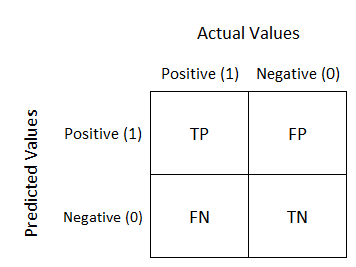
\includegraphics[width=0.3\linewidth]{imgs/conf_matrix}
		\end{figure}
	    На основе этой матрицы есть большое количество разных метрик: \textit{accuracy}, \textit{recall}, \textit{precision}, $F_\beta$, \textit{ROC--AUC}
	\end{frame}

	\begin{frame}
		\frametitle{Классификация: типы классов}
		\begin{itemize}
			\item По количеству классов:
			\begin{itemize}
				\item бинарная классификация
				\item многоклассовая классификация
			\end{itemize}
			\item По пересечению классов 
			\begin{itemize}
				\item пересекающиеся
				\item непересекающаяся
				\item нечёткие
			\end{itemize}
		\end{itemize}
	\end{frame}

	\begin{frame}
		\frametitle{Классификация: этапы обучения модели}
		\begin{itemize}
			\item Выбор модели (класс рассматриваемых $\Phi$ из \ref{3})
			\item Выбор метрики
			\item Выбор метода обучения (способ подбора параметров для минимизации метрики на обучающем множестве)
			\item Выбор метода проверки (способ оценки качества модели)
		\end{itemize}
	\end{frame}

	\begin{frame}
		\frametitle{Классификация: задача оптимизации}
		\begin{itemize}
			\item $\hat{\beta}$ --- параметры модели
			\item $\bm{\Phi}(\bm{x}, \beta)$ --- функционал классификации
			\item $\mathfrak{L}(\bm{\Phi}(\bm{x}, \beta), \bm{y})$ --- функция потерь (метрика)
		\end{itemize}
		\begin{block}{}
			$$\hat{\beta} = \arg\min_{\beta} \mathfrak{L}(\bm{\Phi}(\bm{x}, \beta), \bm{y})$$
		\end{block}
	\end{frame}

	\begin{frame}
		\frametitle{Классификация: отступы}
		Можно ввести ту же задачу через оптимизацию функции от отступов.
		\begin{figure}
			\centering
			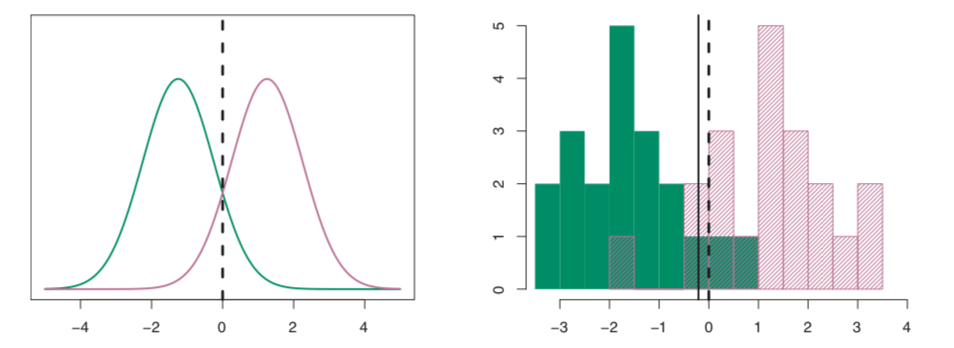
\includegraphics[width=0.7\linewidth]{imgs/margins}

			\label{fig:margins}
		\end{figure}
	\end{frame}

	\begin{frame}
		\frametitle{Классификация: общий подход к решению}
		Как построить функционал $\Phi$?
		
		
		Общий подход --- построить набор $f_i$, $i = 1, \ldots, K$. Каждая функция $f_i(\bm{x})$ показывает меру принадлежности $\bm{x}$ классу $i$. 
		
		Таким образом,
		\begin{equation}
			\Phi(\bm{x}) = \arg\max_i(f_i(\bm{x})).
			\label{4}
		\end{equation}
	\end{frame}
	\begin{frame}
		\frametitle{Дискриминантный анализ}
		Примем за функции $f_i$ из \ref{4} оценку вероятности принадлежности к $i$-му классу.
		
		$$\Phi(\bm{x}) = \arg\max_i (P(C_i|\bm{x})).$$
		
		$C_i$ ---  класс, состоящий из одного события: $\bm{x}$ принадлежит $i$-му классу.
	\end{frame}
	\begin{frame}
		\frametitle{Дискриминантный анализ}
		Если известны априорные вероятности получения $i$-го класса ($\pi_i$), применим формулу Байеса
		
		$$P(C_i|\bm{x}) = {{\pi_i P(\bm{x}|C_i)}\over{\sum_{j=1}^{K} \pi_j P(\bm{x}|C_j)}}.$$
		 
		 Отбросим знаменатель
		
		$$f_i = P(C_i|\bm{x}) = \pi_i P(\bm{x}|C_i).$$
	\end{frame}
	\begin{frame}
		\frametitle{LDA}
		\textit{Предположение:}	
		$$\mathtt{P}(\bm{\xi}|\eta = A_i) = \mathtt{N}(\bm{\mu}_i, \bm{\Sigma})$$
		
		\textit{Классифицирующая функция:}
		$$f_i(\bm{x}) = {{\pi_i}\over{(2\pi)^{p/2}|\bm{\Sigma}|^{1/2}}}exp\left(-{{1}\over{2}}(\bm{x} - \bm{\mu}_i)\bm{\Sigma}^{-1}(\bm{x} - \bm{\mu}_i)^\mathtt{T}\right)$$
		
		\textit{После упрощения:}
		$$h_i(\bm{x}) = -0.5 \bm{\mu}_i\bm{\Sigma}^{-1}\bm{\mu}_i^\mathtt{T} + \bm{\mu}_i\bm{\Sigma}^{-1}\bm{x} + \log\pi_i$$

	\end{frame}

	\begin{frame}
		\frametitle{QDA}
		\textit{Предположение:}	
		$$\mathtt{P}(\bm{\xi}|\eta = A_i) = \mathtt{N}(\bm{\mu}_i, \bm{\Sigma}_i)$$
		
		\textit{Классифицирующая функция:}
		$$f_i(\bm{x}) = {{\pi_i}\over{(2\pi)^{p/2}|\bm{\Sigma}_i|^{1/2}}}exp\left(-{{1}\over{2}}(\bm{x} - \bm{\mu}_i)\bm{\Sigma}_i^{-1}(\bm{x} - \bm{\mu}_i)^\mathtt{T}\right)$$
		
		\textit{После упрощения:}
		$$g_i(\bm{x}) = -0.5 (\bm{x} - \bm{\mu}_i)\bm{\Sigma}^{-1}(\bm{x} - \bm{\mu}_i)^\mathtt{T} - 0.5\log|\bm{\Sigma}_i| + \log\pi_i$$
		
	\end{frame}

	\begin{frame}
		\frametitle{Немного про регрессию}
		Обучающая выборка: $\bm{X} \in \mathbb{R}^{n \times p}, \;\;\mathbf{y}\in \mathbb{R}^n$.
		
		\begin{enumerate}
			\item Модель регрессии:
			$$ \hat{\bm{y}} = \bm{\Phi}(\bm{x}, \beta) = \langle \bm{x}, \beta \rangle = \sum\limits_{j=1}^{p} \beta_j x_j , \; \beta \in \mathbb{R}^p$$
			
			\item Функция потерь:
			$$ \mathfrak{L}(\hat{\bm{y}}, \bm{y}) = (\hat{\bm{y}} - \bm{y})^2$$
			
			
			\item Метод обучения --- метод наименьших квадратов:
			$$ Q(\beta) = \sum\limits_{i = 1}^{n} (\bm{\Phi}(\bm{x}_i, \beta) - \bm{y}_i)^2 \rightarrow \min\limits_{\beta} $$
			
		\end{enumerate}
	\end{frame}
	
	
	\begin{frame}
		\frametitle{Со стороны классификации}
		Обучающая выборка: $\bm{X} \in \mathbb{R}^{n\times p}, \;\; y \in \{-1, 1\}$.
		
		\begin{enumerate}
			\item Модель классификации:
			$$ \hat{y} = \bm{\Phi}(\bm{x}, \beta) = sign \langle \bm{x}, \beta \rangle = sign \sum\limits_{j=1}^{p} \beta_j x_j , \; \beta \in \mathbb{R}^p$$
			
			\item Функция потерь:
			$$ \mathfrak{L}(\hat{y}, y) = [\hat{y} y < 0] = [ \langle \bm{x}, \beta \rangle y < 0 ] \leqslant \hat{\mathfrak{L}}( \langle \bm{x}, \beta \rangle y) $$
			
			
			\item Метод обучения --- минимизация эмпирического риска:
			$$ Q(\beta) = \sum\limits_{i = 1}^{n} [\langle \bm{x}_i, \beta \rangle y_i < 0] \leqslant \sum\limits_{i = 1}^{n} \hat{\mathfrak{L}}( \langle \bm{x}_i, \beta \rangle y_i)  \rightarrow \min\limits_{\beta} $$
			
		\end{enumerate}
	\end{frame}

	\begin{frame}
		\frametitle{Отступы}
		
		$\bm{\Phi}(\bm{x}, \beta) = sign  (g(\bm{x}, \beta))$ --- разделяющий классификатор,\\
		$g(\bm{x}, \beta)$ --- разделяющая функция,\\
		$g(\bm{x}, \beta) = 0$ --- уравнение разделяющей поверхности.\\
		
		\bigskip
		
		$M_i(\beta) = g(\bm{x}_i, \beta) y_i$ --- отступ объекта $\bm{x}_i$. \\
		Если $M_i(\beta) < 0$, тогда алгоритм ошибается на $\bm{x}_i$.
	
	\end{frame}

	\begin{frame}
		\frametitle{Отступы}
		\begin{figure}
			\centering
			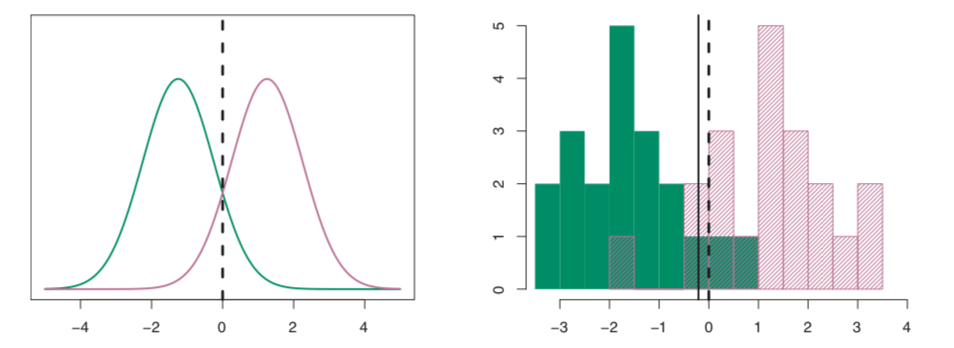
\includegraphics[width=0.7\linewidth]{imgs/margins}
			
			\label{fig:margins}
		\end{figure}
	\end{frame}

	\begin{frame}
	\frametitle{Логистическая регрессия}
	
			Линейная модель классификации для двух классов $y \in \{-1, 1\}$: 
			
			$$ \bm{\Phi}(\bm{x}, \beta) = sign  (\langle \bm{x}, \beta \rangle) $$
			
			Отступ $M = \langle \bm{x}_i, \beta \rangle y$.
			
			Логистическая функция потерь: $\mathfrak{L}(M) = \log (1 + e^{-M})$
			
			Модель условной вероятности: $ P(y| \bm{x}, \beta) = \sigma(M) = \dfrac{1}{1+e^{-M}}$ 
		
	\end{frame}

	\begin{frame}
		\frametitle{Логистическая регрессия: SoftMax}
		Линейный классификатор при произвольном числе классов $|Y|$:
		
		$$\bm{\Phi}(\bm{x}, \beta) = \arg \max\limits_{y \in Y} \langle \bm{x}, \beta_y \rangle $$
		
		Вероятность того, что объект $\bm{x}$ относится к классу $y$:
		
		$$ P(y| \bm{x}, \beta) = \dfrac{e^{\langle \bm{x}, \beta_y \rangle}}{\sum\limits_{z \in Y} e^{\langle \bm{x}, \beta_z \rangle}} = SoftMax_{y \in Y}\langle \bm{x}, \beta_y \rangle $$
		
		Функция $SoftMax: \mathbb{R}^Y \rightarrow \mathbb{R}^Y$ переводит произвольный вектор в нормированный вектор дискретного распределения.
	\end{frame}


	\begin{frame}
		\frametitle{SVM: Постановка задачи}
	
		Выборка: $\{x_i, y_i\}_{i=1}^{n}, \bm{x}_i \in \mathbb{R}^{p}, y_i \in \{-1, 1\}$. \\
		Задача построить классифицирующие правило.\\
		
		\bigskip 
		
		Предположим, что данные - разделимы гиперплоскостью,
		$$ \bm{x}^T\beta - \beta_0 = 0; \beta \in  \mathbb{R}^{p}, \beta_0 \in \mathbb{R},$$
		$$ g(x) =  \bm{x}^T \beta - \beta_0, $$
		$$ \bm{\Phi}(x) =  sign ( g(x) ).$$
	
	\end{frame}

	\begin{frame}
		\frametitle{SVM: Постановка задачи}
		
		Критерий оптимальности: максимальное расстояние между двумя гиперплоскостями, параллельных данной и симметрично расположенных относительно нее.
		
		\bigskip 
		
		Эта пара гиперплоскостей может быть описана парой уравнений:
		$$ \bm{x}^T \beta - \beta_0 = -1, $$
		$$ \bm{x}^T \beta - \beta_0 = 1. $$
		
		\bigskip 
		
		Растояние между ними: $ \dfrac{2}{||\beta||}. $
	\end{frame}

	\begin{frame}
		\frametitle{SVM: Задача квадратичного программирования}
		Принадлежность точек обучающей выборки полупространства описывается
		
		$$ M_i = (\bm{x}^T \beta -  \beta_0) y_i \geqslant 1 $$
		
		Задача сводится к задаче квадратичного программирования с линейными ограничениями:
		
		 $$
			 \begin{cases}
			 	\frac{1}{2}||\beta||_2^2\rightarrow \min\limits_{\beta,\beta_0} \\
			 	M_i  \geqslant 1 \\
			 \end{cases}
		 $$
	
		Случай когда нету линейной разделимости:
		$$
		\begin{cases}
			\frac{1}{2}||\beta||_2^2 + C \sum \xi_i \rightarrow \min\limits_{\beta,\beta_0, \xi} \\
			M_i \geqslant 1 - \xi_i \\
			\xi_i \geqslant 0 \\
		\end{cases}
		$$
	\end{frame}

	\begin{frame}
		\frametitle{SVM: Условия Каруша-Куна-Таккера}
		
		Применение условий Каруша-Куна-Таккера к задаче SVM
		
		Функция Лагранжа: $L(\beta, \beta_0, \xi; \lambda, \eta) =  \frac{1}{2} ||\beta||^2 - \sum\limits_{i=1}^{n}(M_i - 1) - \sum\limits_{i=1}^{n} \xi_i(\lambda_i + \eta_i - C),$
		
		$\lambda_i$ --- переменные, двойственные к ограничениям $M_i \geqslant 1 - \xi_i$,
		
		$\eta_i$ --- переменные, двойственные к ограничениям $\xi_i \geqslant 0 $.
		
			$$
		\begin{cases}
			\dfrac{\partial L}{\partial \beta} = 0, \dfrac{\partial L}{\partial \beta_0} = 0, \dfrac{\partial L}{\partial \xi} = 0; \\
			\xi_i \geqslant 0, \lambda_i \geqslant 0, \eta_i \geqslant 0, i = 1, \dotsc, n; \\
			\lambda_i = 0 \text{ либо } M_i = 1 - \xi_i, i = 1, \dotsc, n; \\
			\eta_i = 0 \text{ либо } \xi_i = 0, i = 1, \dotsc, n;
		\end{cases}
		$$
	
	\end{frame}
	\begin{frame}
		\frametitle{SVM}
		Необходимые условия седловой точки функции Лагранжа:
		$$ 	\dfrac{\partial L}{\partial \beta} = \beta - \sum\limits_{i=1}^{n}\lambda_i y_i \bm{x}_i = 0 \Longrightarrow \beta = \sum\limits_{i=1}^{n}\lambda_i y_i \bm{x}_i $$
		$$ 	\dfrac{\partial L}{\partial \beta_0} = - \sum\limits_{i=1}^{n}\lambda_i y_i = 0 \Longrightarrow \sum\limits_{i=1}^{n}\lambda_i y_i = 0 $$
		$$ 	\dfrac{\partial L}{\partial \xi_i} = \lambda_i - \eta_i - C = 0 \Longrightarrow \lambda_i + \eta_i = C, i = 1, \dotsc, n; $$
	
	\end{frame}
	
	\begin{frame}
		\frametitle{SVM: Опорные объекты}
		Типизация объектов:
		\begin{enumerate}
			\item $ \lambda_i = 0; \eta_i = C; \xi = 0; M_i \geqslant 1 $ - неинформативные объекты.
			\item $ 0 < \lambda_i < C; 0 < \eta_i < C; \xi = 0; M_i = 1 $ - опорные граничные объекты.
			\item $ \lambda_i = C; \eta_i = 0; \xi > 0; M_i < 1 $ - опорные-нарушители.
			
		\end{enumerate}
	
	\bigskip
	
	Объект называется опорным, если $\lambda_i \neq 0$.
		
	\end{frame}

	\begin{frame}
	\frametitle{SVM}
	
	Решаем: 
	$$
		\begin{cases}
			-L(\bm{\lambda}) = - \sum\limits_{i=1}^n \lambda_i + \frac{1}{2} \sum\limits_{i=1}^{n}\sum\limits_{j=1}^{n} \lambda_i \lambda_j y_i y_j (x_i, x_j) \rightarrow \min\limits_{\bm{\lambda}}; \\
			0 \leqslant \lambda_i \leqslant C, i = 1, \dotsc, n; \\
			\sum\limits_{i=1}^{n} \lambda_i y_i = 0.
		\end{cases}
	$$
	
	Подставим полученные $\lambda$:
	
	$$
	\begin{cases}
		\beta = \sum\limits_{i=1}^n \lambda_i y_i x_i;\\
		\beta_0 = \langle\beta, \bm{x}_i\rangle - y_i, \text{ для любого } i: \lambda_i > 0, M_i = 1.
	\end{cases}
	$$
	
	Линейный классификатор: $ \bm{\Phi}(x) = sign ( \sum\limits_{i=1}^{n} \lambda_i y_i \langle\bm{x}, \bm{x}_i\rangle - \beta_0) $
	\end{frame}	
	
	\begin{frame}
		\frametitle{SVM: Нелинейное обобщение}
		Заменим $\langle \bm{x}, \bm{x}^{'} \rangle$ нелинейной функцией $K(\bm{x}, \bm{x}^{'})$.
		
		\begin{block}{Определение}
			Функция $K: X \times X \rightarrow \mathbb{R}$ --- ядро, если $K(\bm{x}, \bm{x}^{'}) = \langle \phi(\bm{x}), \phi(\bm{x}^{'}) \rangle$ при некотором $\phi: X \rightarrow H$, где $H$ --- гильбертово пространство.
		\end{block}
	\end{frame}

	\begin{frame}
		\frametitle{SVM: Примеры ядер}
		\begin{enumerate}
			\item $K(\bm{x}, \bm{x}^{'}) = \langle\bm{x}, \bm{x}^{'} \rangle^2$ --- квадратичное ядро. 
			\item $K(\bm{x}, \bm{x}^{'}) = \langle \bm{x}, \bm{x}^{'} \rangle^d$ --- полиномиальное ядро степени d. 
			\item $K(\bm{x}, \bm{x}^{'}) = \exp(-\gamma ||\bm{x} -  \bm{x}^{'}||^2) $ --- сеть радиальных базисных функций (RBF ядро).
		\end{enumerate}
	\end{frame}

	\begin{frame}
		\frametitle{Кросс-валидация}
		Кросс-валидация (aka перекрестная проверка, скользящий контроль) --- процедура эмпирического оценивания обобщающей способности алгоритмов. 
		
		С помощью кросс-валидации "эмулируется" наличие тестовой выборки, которая не участвует в обучении модели, но для которой известны правильные ответы.
		
	\end{frame}
	\begin{frame}
		\frametitle{Кросс-валидация: виды}
		\begin{itemize}
			\item Валидация на отложенных данных (Hold-Out Validation);
			\item Полная кросс-валидация (Complete Cross-Validation);
			\item k-fold Cross-Validation;
			\item t$\times$k-fold Cross Validation;
			\item Кросс-валидация по отдельным объектам (Leave-One-Out);
			\item Случайные разбиения (Random Subsampling).
		\end{itemize}
		
	\end{frame}

	\begin{frame}
		\frametitle{Кросс-валидация: Обозначения}
		Введем обозначения:
		\begin{itemize}
			\item $\bm{X}$ --- матрица признаков, описывающие таргеты $\bm{y}$;
			\item $\bm{T}^N = (x_i, y_i)_{i=1}^N, x_i \in \bm{X}, y_i \in \bm{y}$ --- обучающая выборка;
			\item $\mathfrak{L}$ --- функция потерь (мера качества);
			\item $A$ --- исследуемая модель;
			\item $\mu : (\bm{X}\times\bm{y})\rightarrow A$ --- алгоритм обучения.
		\end{itemize}
	\end{frame}
	\begin{frame}
		\frametitle{Кросс-валидация: Hold-Out Validation}
		Обучающая выборка один раз случайным образом разбивается на две части $\bm{T} = \bm{T}^t \cup \bm{T}^{N-t}$.
		\begin{figure}
			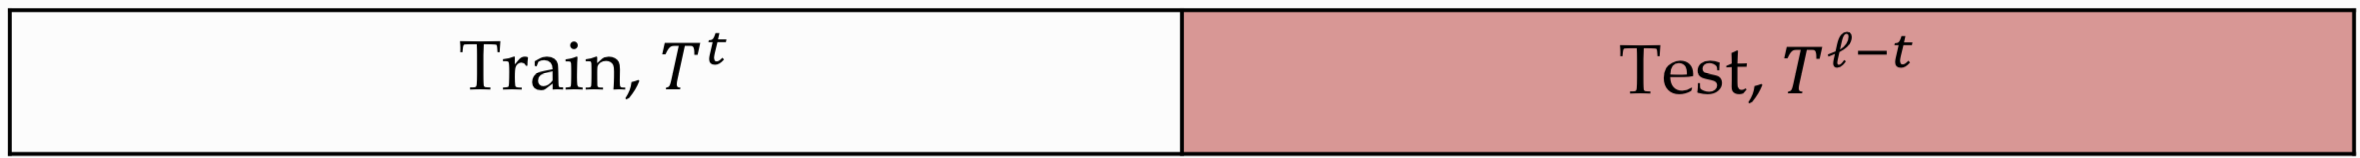
\includegraphics[width=0.9\linewidth]{imgs/hold-out}
		\end{figure}
		После чего решается задача оптимизации:
		$HO(\mu, \bm{T}^t, \bm{T}^{N-t}) = \mathfrak{L}(\mu(\bm{T}^t), \bm{T}^{N-t}) \rightarrow min$.
		
		
		Метод Hold-out применяется в случаях больших датасетов, т.к. требует меньше вычислительных мощностей по сравнению с другими методами кросс-валидации. 
		
		Недостатком метода является то, что оценка существенно зависит от разбиения, тогда как желательно, чтобы она характеризовала только алгоритм обучения.
	\end{frame}

	\begin{frame}
		\frametitle{Кросс-валидация: Complite cross-validation}
		\begin{itemize}
			\item Выбирается значение $t$;
			\item Выборка разбивается всевозможными способами на две части $\bm{T} = \bm{T}^t \cup \bm{T}^{N-t}$.
		\end{itemize}
		\begin{figure}
			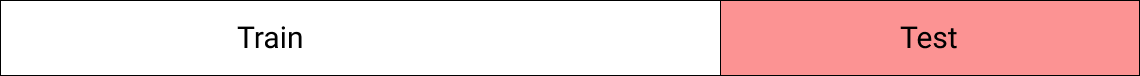
\includegraphics[width=0.9\linewidth]{imgs/completecrossvalidation}
		\end{figure}
		После чего решается задача оптимизации:
		$CVV_t = \frac{1}{C_N^{N-t}}\sum\limits_{\bm{T}^N = \bm{T}^t \cup \bm{T}^{N-t}} \mathfrak{L}(\mu(\bm{T}^t), \bm{T}^{N-t}) \rightarrow min$.
		
		
		Здесь число разбиений $ C_N^{N-t} $ становится слишком большим даже при сравнительно малых значениях $ t $, что затрудняет практическое применение данного метода.
	\end{frame}

    \begin{frame}
		\frametitle{Кросс-валидация: k-fold Cross-Validation}
		\begin{itemize}
			\item $\bm{T}^N$ разбивается на $ \bm{T_1}\cup\cdots\cup\bm{T_k}, |\bm{T_i}|\approx \frac{1}{k} $ частей;
			\item Производится $ k $ итераций:
			\begin{itemize}
				\item Модель обучается на $ k-1 $ части обучающей выборки;
				\item Модель тестируется на части обучающей выборки, которая не участвовала в обучении.
			\end{itemize}
		\end{itemize}
		Каждая из $ k $ частей единожды используется для тестирования.
		
		\begin{figure}
			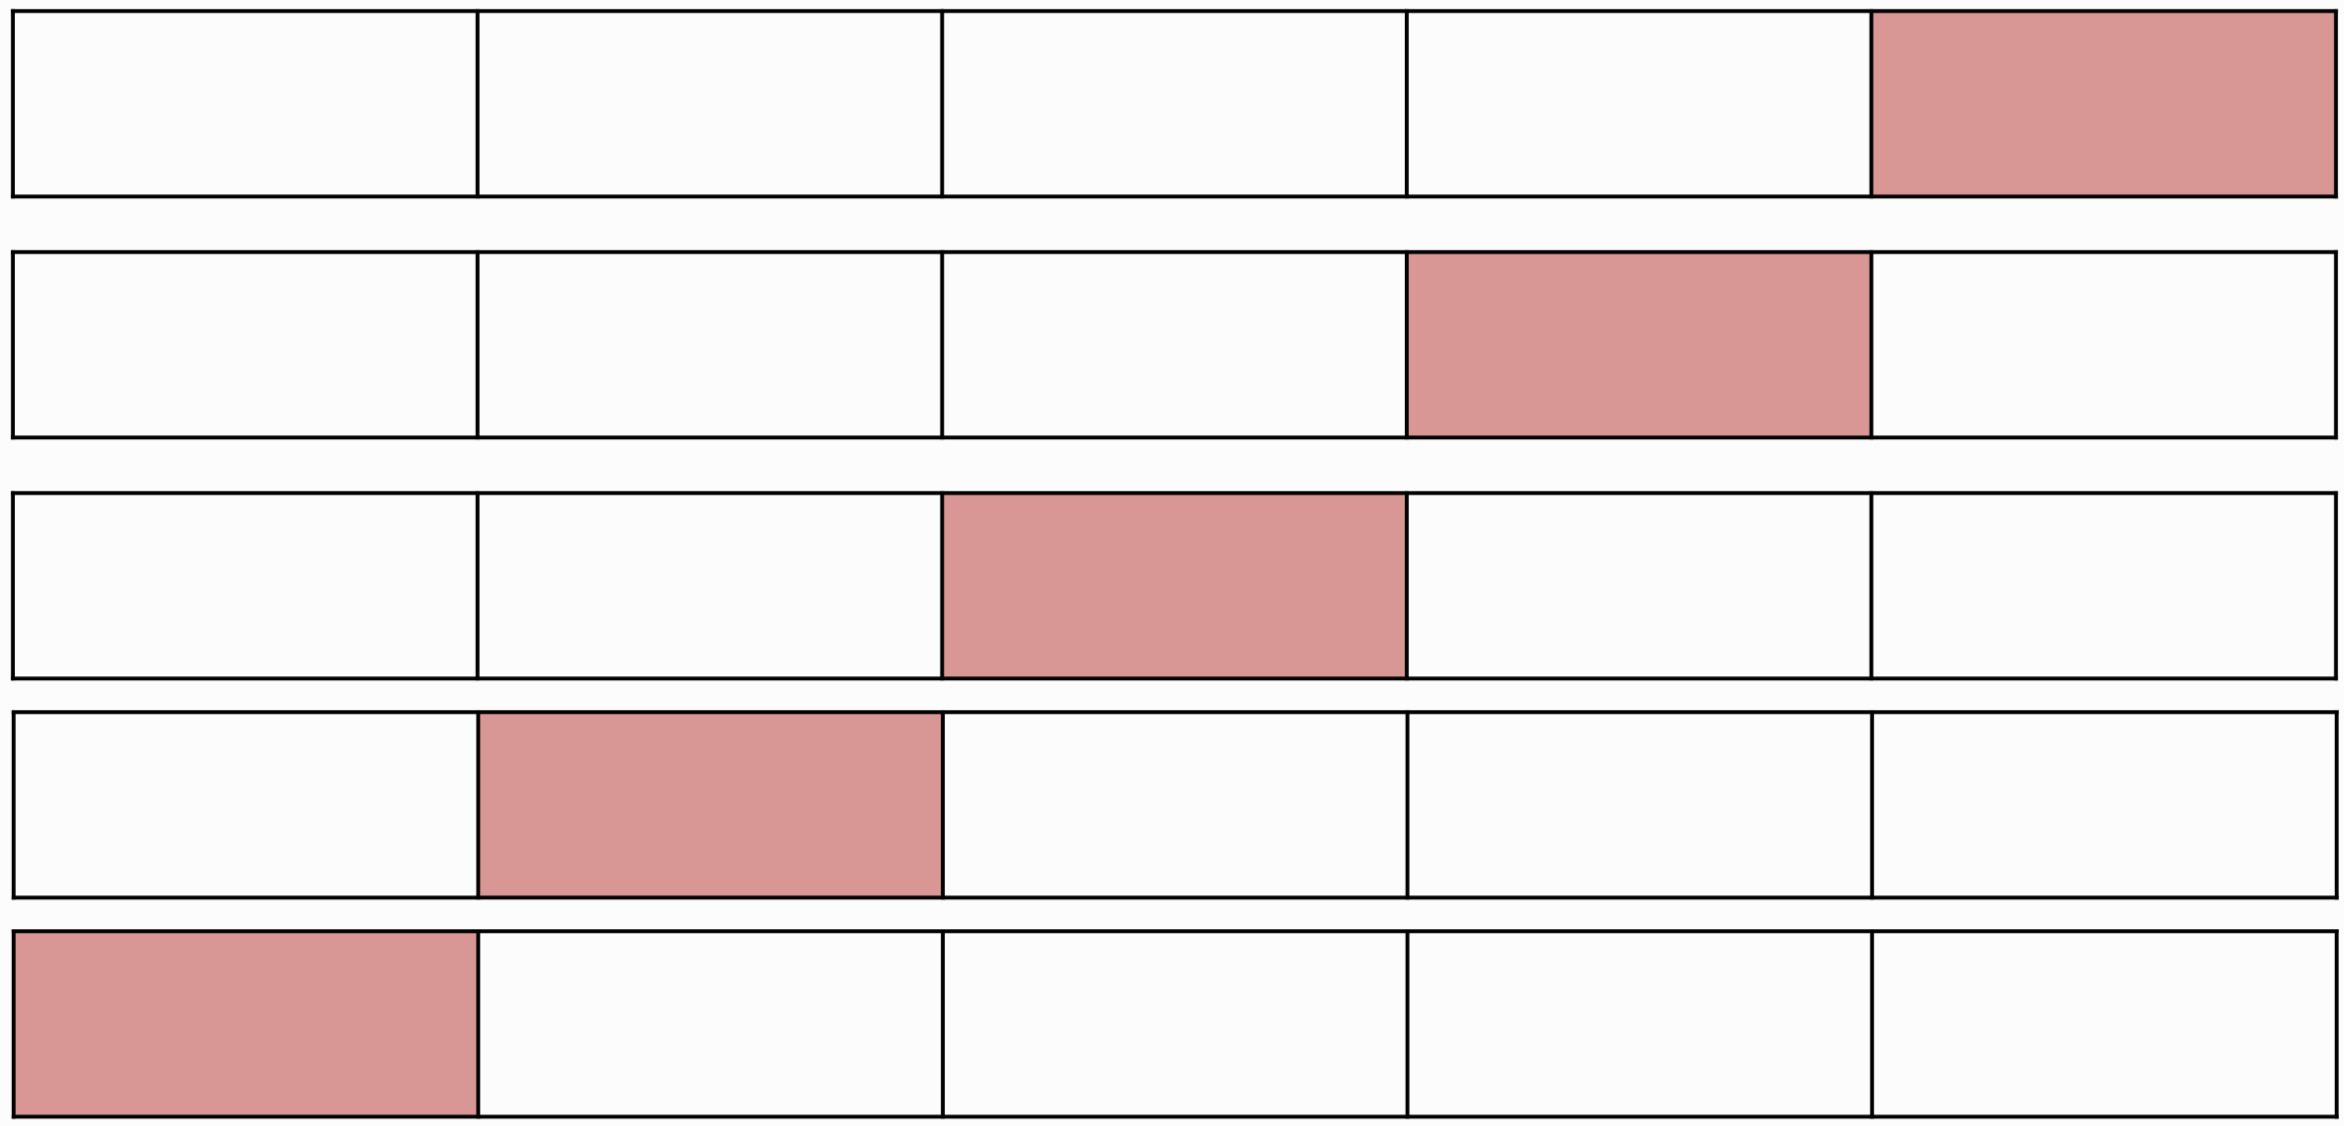
\includegraphics[width=0.4\linewidth]{imgs/K-fold-validation}
		\end{figure}
		После чего решается задача оптимизации:
		$CV_k = \frac{1}{k}\sum\limits_{i=1}^k\mathfrak{L}(\mu(\bm{T}^N \setminus \bm{T}_i), \bm{T}_i) \rightarrow min$.
	\end{frame}

	\begin{frame}
		\frametitle{Кросс-валидация: t$\times$k-fold Cross Validation}
		\begin{center}
			\textit{Как k-fold Cross-Validation, только $t$ раз.}
		\end{center}
		
		Разбиение:
		$\bm{T}^N = \bm{T}_{(1,1)}\cup\cdots\cup\bm{T}_{(k,1)}=\bm{T}_{(1,t)}\cup\cdots\cup\bm{T}_{(k,t)},|\bm{T}_{(i,j)}|\approx \frac{N}{k} $, 
		 
		Задача оптимизации: 
		$CV_{t\times k} = \frac{1}{tk}\sum\limits_{j=1}^t\sum\limits_{i=1}^k\mathfrak{L}(\mu(\bm{T}^N \setminus \bm{T}_{(i,j)}), \bm{T}_{(i,j)}) \rightarrow min$
	\end{frame}

	\begin{frame}
		\frametitle{Кросс-валидация: Leave-One-Out}
		Выборка разбивается на $ N-1 $ и $ 1 $ объект $ N $ раз.
		$LOO = \frac{1}{N}\sum\limits_{i=1}^N\mathfrak{L}(\mu(\bm{T}^N \setminus p_i), p_i) \rightarrow min$, где $ p_i = (x_i, y_i) $.
		
		Преимущества LOO в том, что каждый объект ровно один раз участвует в контроле, а длина обучающих подвыборок лишь на единицу меньше длины полной выборки.
		
		Недостатком LOO является большая ресурсоёмкость, так как обучаться приходится $ N $ раз.
	\end{frame}

	\begin{frame}
		\frametitle{Кросс-валидация: Random subsampling (Monte-Carlo cross-validation)}
		Выборка разбивается в случайной пропорции. Процедура повторяется несколько раз.
		\begin{figure}
			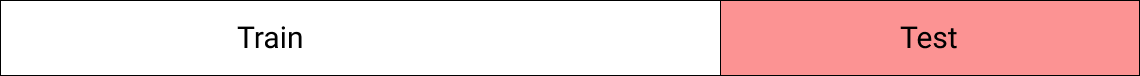
\includegraphics[width=1\linewidth]{imgs/completecrossvalidation}
		\end{figure}
	\end{frame}
	
	\begin{frame}
		\frametitle{Кросс-валидация: Выбор лучшей модели}
		Не переобученый алгоритм должен показывать одинаковую эффективность на каждой части.
		
	\end{frame}

	\begin{frame}
		\frametitle{SGD}
		Стохастический градиентный спуск - оптимизационный алгоритм, при котором градиент оптимизируемой функции считается на каждой итерации от случайно выбранного элемента выборки.
	\end{frame}
	\begin{frame}
		\frametitle{Вспомним про GD: обозначения}
		\begin{itemize}
			\item $ \bm{X} \in \mathrm{R}^{n\times p} $ --- матрица признаков;
			\item $ y^*:\bm{X}\rightarrow\bm{y} $ - целевая зависимость, известная на $ \bm{X}^l $;
			\item $ \bm{y} = y^*(\bm{X}) \in  \mathrm{A}^n $ --- вектор классовой принадлежности;
			\item $ \bm{X}^l $ --- обучающая выборка, состоящая из пар $ (x_i, y_i)_{i=1}^l $;
			\item $ a(x, \omega) $ --- семейство алгоритмов с параметром вектора весов $ \omega $;
			\item $ \mathfrak{L}(a, y) $ --- функция потерь, выбранная из класса $ C_1 $.
			
		\end{itemize}
		
	\end{frame}
	
	\begin{frame}
		\frametitle{Вспомним про GD: постановка задачи}
		Найдем алгоритм $ a(x, \omega) $, аппроксимирующий зависимость $ y^* $.
		
		Например, в случае линейного классификатора искомый алгоритм имеет вид:
		$$ a(x, \omega) = \phi(\sum\limits_{j=1}^N \omega_jx^j - \omega_0), $$где $ \phi(z) $ - функция активации. 
		
		\textit{Решаемая задача оптимизации:}
		$$ Q(\omega) = \frac{1}{N}\sum\limits_{i=1}^{N}\mathfrak{L}(a(x_i, \omega), y_i)\rightarrow\min\limits_{\omega} $$
		\textit{Обновление весов:}
		$$ \omega^{(t+1)} = \omega^{(t)} - h\nabla Q(\omega^{(t)}) $$
		
	\end{frame}

	
	\begin{frame}
		\frametitle{Вспомним про GD: Проблемы}
		Проблема GD --- чтобы определить новое приближение вектора весов необходимо вычислить градиент от каждого элемента выборки, что может сильно замедлять алгоритм.
		Идея ускорения заключается в использовании либо одного элемента (SGD), либо некоторой подвыборки (Batch GD) для получения нового приближения весов. 
		
		
		
	\end{frame}

	\begin{frame}
		\frametitle{Ускоряем GD - SGD}
		\textit{Веса, при подходе SGD, обновляются следующим образом:}
		
		$$ \omega^{(t+1)} = \omega^{(t)} - h\nabla\mathfrak{L}(a(x_i, \omega^{(t)}), y_i),$$ где $ i $ --- случайно выбранный индекс.
		
		Т.к. направление изменения $ \omega $ будет определяться за $ O(1) $, подсчет $ Q $ на каждом шаге будет слишком дорогостоящим. Для ускорения оценки, будем использовать одну из рекуррентных формул:
		\begin{itemize}
			\item Среднее арифметическое: $ \overline Q_m = \frac{1}{m}\mathfrak{L}(a(x_{i_m}, \omega^{(m)}), y_{i_m}) + (1 - \frac{1}{m}) \overline Q_{m-1}$;
			\item Экспоненциальное скользящее среднее: $ \overline Q_m = \lambda\mathfrak{L}(a(x_{i_m}, \omega^{(m)}), y_{i_m}) + (1 - \lambda) \overline Q_{m-1}$, где $ \lambda $ --- темп забывания "предыстории" ряда.
		\end{itemize}
	\end{frame}

	\begin{frame}
		\frametitle{SGD: А что с инициализацией весов?}
		Существует несколько способов:
		\begin{itemize}
			\item $ \omega = 0 $;
			\item $ \omega_j = random(-\frac{1}{2n}, \frac{1}{2n}) $;
			\item $ \omega_j = \frac{\langle y, x_j \rangle}{\langle x_j, x_j \rangle} $, если признаки независимы, функция активации линейна, а функция потерь квадратична.
		\end{itemize}
	\end{frame}

	\begin{frame}
		\frametitle{SGD: А что со сходимостью?}
		Установлено, что если скорость обучения убывает при увеличении числа итераций SGD сходится почти наверняка к глобальному минимуму в случае выпуклой или псевдовыпуклой функции $ Q(\omega) $, в противном случае метод сходится почти наверняка к локальному минимуму.
	\end{frame}

	\begin{frame}
		\frametitle{SGD: Достоинства и недостатки}
		Достоинства:
		\begin{itemize}
			\item Легко реализуется;
			\item Функция потерь и семейство алгоритмов могут быть любыми (если функция потерь не дифференцируема, ее можно аппроксимировать дифференцируемой);
			\item Легко добавить регуляризацию;
			\item Возможно потоковое обучение;
			\item Подходит для задач с большими данными, иногда можно получить решение даже не обработав всю выборку.
		\end{itemize}
	
		Недостатки:
		\begin{itemize}
			\item Нет универсального набора эвристик, их нужно выбирать для конкретной задачи отдельно;
	 		\item На практике остаются проблемы с локальными экстремумами.
		\end{itemize}
	\end{frame}
	
	\begin{frame}
		\frametitle{Модификации (или о чем можно почитать на досуге)}
		\begin{itemize}
			\item Не выраженные явно изменения (ISGD) --- градиент пересчитывается на следующей итерации;
			\item Метод импульса --- запоминает $ \Delta\omega $ на каждой итерации и определяет следующее изменение в виде линейной комбинации градиента и предыдущего изменения;
			\item Усреднённый стохастический градиентный спуск;
			\item AdaGrad --- модификация SGD с отдельной для каждого параметра скоростью обучения;
			\item RMSProp --- это метод, в котором скорость обучения настраивается для каждого параметра. Идея заключается в делении скорости обучения для весов на скользящие средние значения недавних градиентов для этого веса;
			\item Adam --- это обновление оптимизатора RMSProp. Здесь используются скользящие средние как градиентов, так и вторых моментов градиентов.
			\item Kalman-based SGD.
		\end{itemize}
	\end{frame}
	
\end{document}